\newcounter{english}
\documentclass{article}

% packages
\usepackage{amsmath, amsthm, thmtools, amsfonts, amssymb, luacode, catchfile, tikzducks, hyperref, ifthen}
\ifcsname c@kobocompile\endcsname
	\usepackage[a5paper, total={1072pt, 1448pt}, margin=10pt, includeheadfoot]{geometry} % set page margins
\else
	\usepackage[a4paper, margin=50pt, includeheadfoot]{geometry}
\fi
\usepackage[shortlabels]{enumitem}
\usepackage[skip=3pt, indent=0pt]{parskip}

% language
\usepackage[bidi=basic, layout=tabular, provide=*]{babel}
\ifcsname c@english\endcsname
	\babelprovide[main, import]{english}
\else
	\babelprovide[main, import]{hebrew}
	\babelprovide{rl}
\fi
%\babelfont{rm}{Libertinus Serif}
\babelfont{rm}[Renderer=Harfbuzz]{Libertinus Serif}
\babelfont{sf}{Libertinus Sans}
\babelfont{tt}{Libertinus Mono}

% style
\AddToHook{cmd/section/before}{\clearpage}	% Add line break before section
\linespread{1.3}
\setcounter{secnumdepth}{0}		% Remove default number tags from sections, this won't do well with theorems
\AtBeginDocument{\setlength{\belowdisplayskip}{3pt}}
\AtBeginDocument{\setlength{\abovedisplayskip}{3pt}}
\graphicspath{ {../images/} }

% operators
\DeclareMathOperator\cis{cis}
\DeclareMathOperator\Sp{Sp}
\DeclareMathOperator\tr{tr}
\DeclareMathOperator\im{Im}
\DeclareMathOperator\re{Re}
\DeclareMathOperator\diag{diag}
\DeclareMathOperator*\lowlim{\underline{lim}}
\DeclareMathOperator*\uplim{\overline{lim}}
\DeclareMathOperator\rng{rng}
\DeclareMathOperator\Sym{Sym}
\DeclareMathOperator\Arg{Arg}
\DeclareMathOperator\Log{Log}
\DeclareMathOperator\dom{dom}
\DeclareMathOperator\supp{Supp}
\DeclareMathOperator\var{Var}
\DeclareMathOperator\cov{Cov}

% commands
%\renewcommand\qedsymbol{\textbf{מש''ל}}
%\renewcommand\qedsymbol{\fbox{\emoji{lizard}}}
\newcommand{\Aa}[0]{\mathcal{A}}
\newcommand{\Bb}[0]{\mathcal{B}}
\newcommand{\CC}[0]{\mathbb{C}}
\newcommand{\Cc}[0]{\mathcal{C}}
\newcommand{\EE}[0]{\mathbb{E}}
\newcommand{\FF}[0]{\mathbb{F}}
\newcommand{\Ff}[0]{\mathcal{F}}
\newcommand{\Ii}[0]{\mathcal{I}}
\newcommand{\Gg}[0]{\mathcal{G}}
\newcommand{\Ll}[0]{\mathcal{L}}
\newcommand{\Mm}[0]{\mathcal{M}}
\newcommand{\NN}[0]{\mathbb{N}}
\newcommand{\Nn}[0]{\mathcal{N}}
\newcommand{\PP}[0]{\mathbb{P}}
\newcommand{\Pp}[0]{\mathcal{P}}
\newcommand{\QQ}[0]{\mathbb{Q}}
\newcommand{\RR}[0]{\mathbb{R}}
\newcommand{\Rr}[0]{\mathcal{R}}
\newcommand{\Ss}[0]{\mathcal{S}}
\newcommand{\TT}[0]{\mathbb{T}}
\newcommand{\Uu}[0]{\mathcal{U}}
\newcommand{\Vv}[0]{\mathcal{V}}
\newcommand{\Ww}[0]{\mathcal{W}}
\newcommand{\ZZ}[0]{\mathbb{Z}}
\newcommand{\acts}[0]{\circlearrowright}
\newcommand{\explain}[2] {
	\begin{flalign*}
		 && \text{#2} && \text{#1}
	\end{flalign*}
}
\newcommand{\maketitleprint}[0]{ \begin{center}
	%\begin{tikzpicture}[scale=3]
	%	\duck[graduate=gray!20!black, tassel=red!70!black]
	%\end{tikzpicture}	
	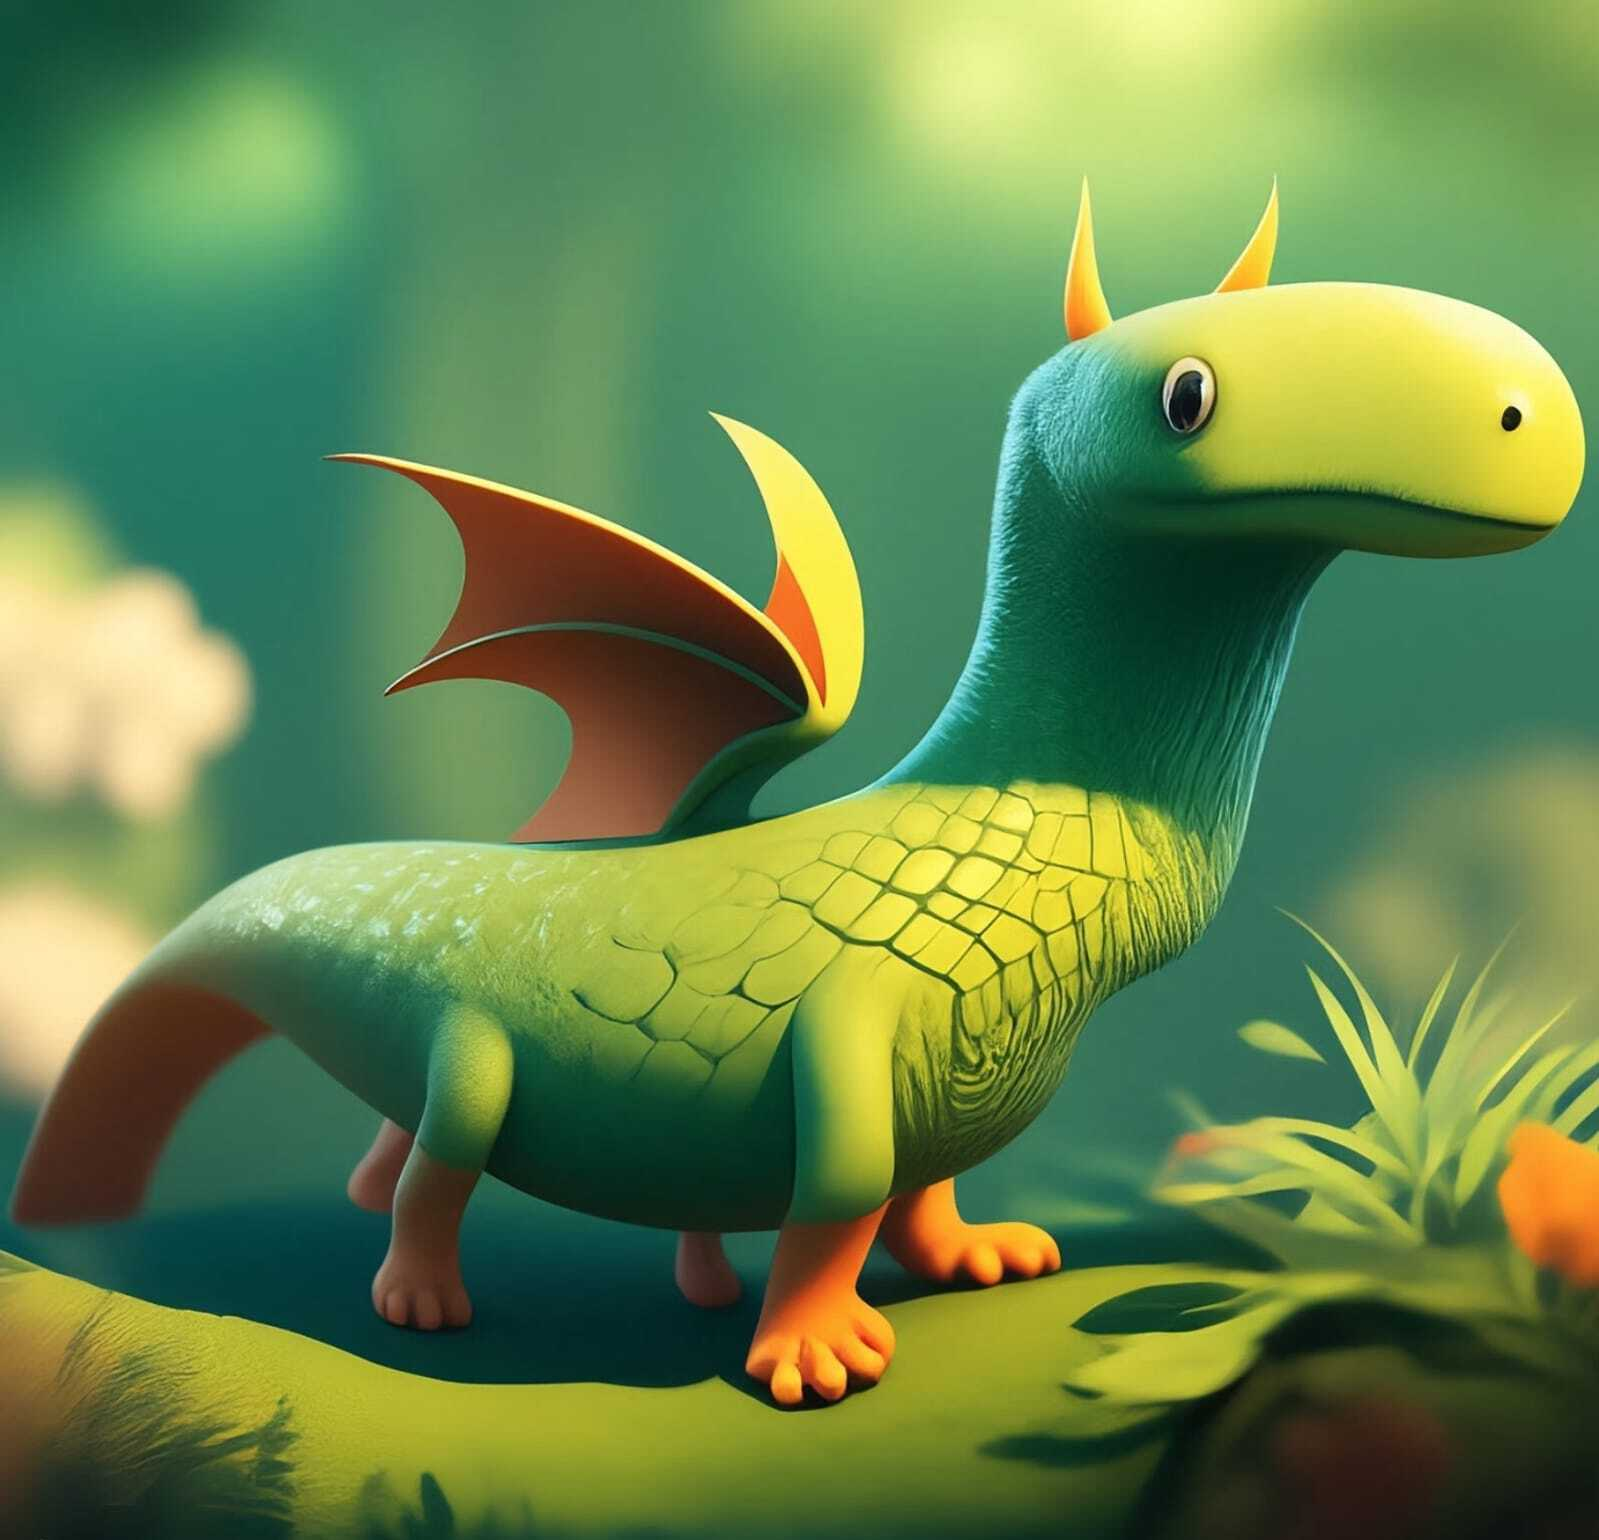
\includegraphics[width=6cm]{cover}
\end{center}
}

% theorem commands
\newtheoremstyle{c_remark}
	{}	% Space above
	{}	% Space below
	{}% Body font
	{}	% Indent amount
	{\bfseries}	% Theorem head font
	{}	% Punctuation after theorem head
	{.5em}	% Space after theorem head
	{\thmname{#1}\thmnumber{ #2}\thmnote{ \normalfont{\text{(#3)}}}}	% head content
\newtheoremstyle{c_definition}
	{3pt}	% Space above
	{3pt}	% Space below
	{}% Body font
	{}	% Indent amount
	{\bfseries}	% Theorem head font
	{}	% Punctuation after theorem head
	{.5em}	% Space after theorem head
	{\thmname{#1}\thmnumber{ #2}\thmnote{ \normalfont{\text{(#3)}}}}	% head content
\newtheoremstyle{c_plain}
	{3pt}	% Space above
	{3pt}	% Space below
	{\itshape}% Body font
	{}	% Indent amount
	{\bfseries}	% Theorem head font
	{}	% Punctuation after theorem head
	{.5em}	% Space after theorem head
	{\thmname{#1}\thmnumber{ #2}\thmnote{ \text{(#3)}}}	% head content

\ifcsname c@english\endcsname
	\theoremstyle{plain}
	\newtheorem{theorem}{Theorem}[section]
	\newtheorem{lemma}[theorem]{Lemma}
	\newtheorem{proposition}[theorem]{Proposition}
	\newtheorem*{proposition*}{Proposition}
	%\newtheorem{corollary}[theorem]{אין חלופה עברית}

	\theoremstyle{definition}
	\newtheorem{definition}[theorem]{Definition}
	\newtheorem*{definition*}{Definition}
	\newtheorem{example}{Example}[section]
	\newtheorem{exercise}{Exercise}[section]

	\theoremstyle{remark}
	\newtheorem*{remark}{Remark}
	\newtheorem*{solution}{Solution}
	\newtheorem{conclusion}[theorem]{Conclusion}
	\newtheorem{notation}[theorem]{Notation}
\else
	\theoremstyle{c_plain}
	\newtheorem{theorem}{משפט}[section]
	\newtheorem{lemma}[theorem]{למה}
	\newtheorem{proposition}[theorem]{טענה}
	\newtheorem*{proposition*}{טענה}
	%\newtheorem{corollary}[theorem]{אין חלופה עברית}

	\theoremstyle{c_definition}
	\newtheorem{definition}[theorem]{הגדרה}
	\newtheorem*{definition*}{הגדרה}
	\newtheorem{example}{דוגמה}[section]
	\newtheorem{exercise}{תרגיל}[section]

	\theoremstyle{c_remark}
	\newtheorem*{remark}{הערה}
	\newtheorem*{solution}{פתרון}
	\newtheorem{conclusion}[theorem]{מסקנה}
	\newtheorem{notation}[theorem]{סימון}
\fi

% Questions related commands
\newcounter{question}
\setcounter{question}{1}
\newcounter{sub_question}
\setcounter{sub_question}{1}

\ifcsname c@english\endcsname
	\newcommand{\question}[1][0]{
		\ifthenelse{#1 = 0}{}{\setcounter{question}{#1}}
		\section{Question \arabic{question}}
		\addtocounter{question}{1}
		\setcounter{sub_question}{1}
	}

	\newcommand{\subquestion}[1][0]{
		\ifthenelse{#1 = 0}{}{\setcounter{sub_question}{#1}}
		\subsection{Part \alph{sub_question}}
		\addtocounter{sub_question}{1}
	}
\else
	\newcommand{\question}[1][0]{
		\ifthenelse{#1 = 0}{}{\setcounter{question}{#1}}
		\section{שאלה \arabic{question}}
		\addtocounter{question}{1}
		\setcounter{sub_question}{1}
	}

	\newcommand{\subquestion}[1][0]{
		\ifthenelse{#1 = 0}{}{\setcounter{sub_question}{#1}}
		\subsection{סעיף \localecounter{letters.gershayim}{sub_question}}
		\addtocounter{sub_question}{1}
	}
\fi

% import lua and start of document
\directlua{common = require ('../common')}

\GetEnv{AUTHOR}

% headers
\author{\AUTHOR}
\date\today

\title{Exercise 6 Answer Sheet --- Logic Theory (2), 80424}

\DeclareMathOperator{\PA}{PA}
\DeclareMathOperator{\Coll}{Coll}
\DeclareMathOperator{\Ind}{Ind}

\begin{document}
\maketitle
\maketitleprint[yellow]

\question{}
\begin{notation}[Closure over induction scheme]
	Suppose that $\Gamma$ is some collection of formulas over $L_{\PA}$,
	then we define $I \Gamma = \{ \Ind(\varphi) \mid \varphi \in \Gamma \}$.
\end{notation}
\begin{notation}[Collection formula]
	Suppose that $\varphi(z, y, t_0, \ldots, t_{n - 1})$ is some formula in $L_{\PA}$,
	then we define $\Coll(\varphi) = \forall z \forall t_0 \ldots \forall t_{n - 1} (\forall x \le z \exists y\ \varphi \leftrightarrow \exists w \forall x \le z \exists y \le w\ \varphi)$.
\end{notation}
In the previous exercise we proved that $\PA \vdash \Coll(\varphi)$ for any $\varphi$.
Let $\Coll = \{ \Coll(\varphi) \mid \varphi \in \operatorname{form}_{L_{\PA}} \}$.
Let $Q \subseteq \PA$ be the first 9 axioms without the induction scheme, and let $\PA_0 = Q \cup I \Sigma_0 \cup \Coll$.
We will show that $\PA_0 \vdash I \Sigma_1$.
\begin{proof}
	Let $\psi \in I \Sigma_1$, meaning that $\psi = \Ind(\exists x\ \varphi(x, y, z))$ for some $\varphi \in \Sigma_0$, for localized version of $\Sigma_0$.
	Let us assume that $\Mm \models \PA_0$ is some model such that $c = z^\Mm$ for some $z$ such that $\Mm \models \exists x\ \varphi(x, 0, c)$ and $\Mm \models (\exists x\ \varphi(x, y, c)) \to (\exists x\ \varphi(x, y + 1, c))$.
	There exists such a model as this sentence is satisfiable. \\
	We intend to show that $\Mm \models \forall y \exists x\ \varphi(x, y, c)$.
	We fix some $b \in M$, and want to show that $\Mm \models \exists x \varphi(x, b, c)$.
	We use $\Coll(\varphi(x, y \le b, c))$ to fix some $d$ such that for all $b' \le b$, if $\Mm \models \exists x\ \varphi(x, b', c)$ then $\Mm \models \exists x \le d\ \varphi(x, b', c)$.
	Note that this is an $I \Sigma_0$ formula, thus by our assumptions about $\Mm$ it holds, and it follows that $\exists x \varphi(x, b, c)$ holds as well.
\end{proof}

\question[3]
\subquestion{}
We will show that full recursion functions are definable.
\begin{proof}
	Let us assume that $G$ is some primitive-recursion function, and we define $F(n) = G(\# \langle F(i) \mid i < n \rangle)$ (the sequence is coded).
	We will show that $F$ is primitive recursion definable by showing it is $\Sigma_0^1$. \\
	Note that when given a finite sequence, a function to append value to the sequence is primitive-recursive.
	This is true as the length function is primitive-recursive, as the singleton and union, enabling us to code the pair $\langle i, x \rangle$ for some given $x$ numeral.
	Let $\eta : \NN^2 \to \NN$ be such function, meaning that $\eta(\# \langle a_i \mid i < n \rangle, a_{i + 1}) = \#\langle a_i \mid i < n + 1 \rangle$. \\
	Lastly we define $H(x) = \eta(x, G(x))$ and use the induction scheme over it to define $F$.
\end{proof}

\subquestion{}
We will show that the relation $P(x)$ such that $P(x)$ if and only if $x$ is a prime, is primitive-recursive.
\begin{proof}
	$P(x) \iff \forall y,\ y \mid x \to y = 1 \lor y = x$.
	This is clearly a $\Sigma_0$ formula, thus implies that $P$ is $\Delta_1^0$ and a primitive-recursion relation.
\end{proof}

\subquestion{}
We will show that the function $n \mapsto p_n$ where $p_n$ it the $n$-th prime, is primitive-recursion function.
\begin{proof}
	By primes definition and the order of the primes as sub-order of the elements,
	\[
		F(n + 1) = y
		\iff \exists p_n < y < p_n^2,\ P(y) \land \forall p_n < x < y, \lnot P(y)
	\]
	But this is full recursion using a primitive-recursion relation, then we deduce that $F$ is indeed primitive-recursive.
\end{proof}

\question{}
We define the base $b$-concatenation as the function such that for every $x, y, b \in \NN$, $x *_b y$ is the representation of the digits of $x$ followed by these of $y$ in base $b$.
We will show that the function $(x, y, b) \mapsto x *_b y$ is primitive-recursive.
\begin{proof}
	We define the operation $/$ as the no-residue division, meaning that if $y = x \cdot b + c$ for $c < b$, then $y / b = x$.
	This is a primitive-recursive as it is a $\Sigma_1^0$ function.
	%Let $\%$ be the residue operation, meaning that $y \% b = x$.

	We define the least nullifier function as the function such that $\lambda_b(x)$ is finite product of $b$, that its the minimal value such that $x / \lambda_b(x) = 0$.
	For example, $\lambda_2(7) = 2^3 = 8$.
	We also define $0 \mapsto 1$.
	The recursive definition is 
	\[
		\lambda_b(x)
		= \begin{cases}
			1 & x = 0 \\
			b \cdot \lambda(x / b) & x > 0
		\end{cases}
	\]
	This is a primitive-recursive function by question 3.

	Directly from definition of base-$b$ representation of a number we deduce that $x \cdot \lambda_b(y) + y$ is the concatenation.
\end{proof}

\end{document}
